\documentclass[10pt]{sigplanconf}

\usepackage{amsmath,amssymb, latexsym}
%\usepackage[noend]{algorithmic}
%\usepackage{algorithm}
\usepackage{program}
%\usepackage{pstricks}
\usepackage{graphicx}
\usepackage{wrapfig}
\usepackage{enumerate}
\usepackage{hyperref}
\def\url{}
\usepackage{subfigure}
\usepackage{epsfig}
\usepackage{epic}
\usepackage{eepic}


% command to end a proof or definition:
\def\qed{\rule{0.4em}{1.4ex}}

% space at the beginning of an environment:
\def\@envspa{\hspace{0.3em}}
\def\@sa{\hspace{-0.2em}}
\def\@sb{\hspace{0.5em}}
\def\@sc{\hspace{-0.1em}}
\def\sk{\smallskip}		% space before and after theorems

\newtheorem{notation}{Notation}{\itshape}{}
%\newtheorem{theoremstar}{Theorem}{\bfseries\upshape}{\itshape}
%\newtheorem{@protheo}{Theorem}

%\newenvironment{theorem}[1]{\begin{@protheo}{\rm \bf #1}\it}{\end{@protheo}}
%\newenvironment{proposition}[1]{\begin{@protheo}{\rm \bf #1}\it}{\end{@protheo}}

%\newtheorem{remark}{Remark}{\bfseries\upshape}{\rm}
%\newtheorem{definition}{Definition}{\bfseries\upshape}{\itshape}
% this is from the lazy_abstraction paper
%\newtheorem{notation}{Notation}{\itshape}{}
\newtheorem{theoremstar}{Theorem}{\bfseries\upshape}{\itshape}
\newtheorem{@protheo}{Theorem}
\newenvironment{theorem}[1]{\begin{@protheo}{\rm \bf #1}\it}{\end{@protheo}}
\newtheorem{remark}{Remark}{\bfseries\upshape}{\rm}
\newtheorem{definition}{Definition}{\bfseries\upshape}{\itshape}
\newtheorem{proposition}{Proposition}{\bfseries\upshape}{\itshape}
\newtheorem{lemma}{Lemma}{\bfseries\upshape}{\itshape}
\newtheorem{corollary}{Corollary}{\bfseries\upshape}{\itshape}
\newtheorem{invariant}{Invariant}



\newcounter{ex}
\stepcounter{ex}

\newenvironment{example}{\vspace{0.05in} \noindent {\sc Example \arabic{ex}: }}{\stepcounter{ex} \hfill $\Box$ \vspace{0.05in} }
%\theoremstyle{remark}
%\newtheorem{@proex}{Example}
%\newenvironment{example}[1]{\begin{@proex}{\rm \bf #1}}{\end{@proex                      }}
%\newtheorem{example}{Example}

\def\mynote#1{{\sf $\clubsuit$ #1$\clubsuit$}}

% comment environment
% comment.sty
% 25-Oct-89
% By Ed -- modified from verbatim in /usr/loca/lib/tex82/latex.tex

% \begin{comment}
% \end{comment}

\makeatletter

\begingroup \catcode `|=0 \catcode `[= 1
\catcode`]=2 \catcode `\{=12 \catcode `\}=12
\catcode`\\=12 |gdef|@xcomment#1\end{comment}[|end[comment]]
|endgroup

\def\@comment{\let\do\@makeother \dospecials\catcode`\^^M=10\def\par{}}

\def\begincomment{\@comment\@xcomment}

\makeatother

\newenvironment{comment}{\begincomment}{}


%%%%%%%%%%%%%%%% general macros

\def\set#1{{\{ #1 \}}}

%%%%%%%%%%%%%%%% paper specific macros
\def\Next{\hspace{4pt}\raise 3pt \hbox{\circle{7}} \hspace{4pt} }
\newcommand{\dia}{{\raisebox{-0.2ex}{$\Diamond$}}}
\newcommand{\PastDiamond}                                     % past diamond
     {\mbox{\rm\makebox[0em][l]{$\dia$}\makebox[0.8em]{--}\hspace{0.05em}}}

\def\create{{\mathsf{create}}}

\def\alloc{{\mathsf{alloc}}}
\def\access{{\mathsf{access}}}
\def\delete{{\mathsf{delete}}}

\def\acquire{{\mathtt{acq}}}
\def\release{{\mathtt{rel}}}

\def\alias{{\mathsf{alias}}}
\def\mayalias{{\mathsf{mayAlias}}}
\def\mustalias{{\mathsf{mustAlias}}}

%%%%%%%%%%%%%%%%%%%%%%%%%%%%%%%%%%%%%%%%%%%%%
\sloppy

\begin{document}
\title{Static Checking for Dynamic Resource Management \\ in Sensor
  Network Systems}

\authorinfo{Sensys Paper \#66}

%% \authorinfo{The SOS Reliability Working Group :)}
%% {UCLA}


\maketitle

% -*- tex-main-file: "main.tex" -*-

\begin{abstract}
%
\noindent Many sensor network systems expose general interfaces to
system developers for dynamically creating and manipulating resources
of various kinds.
%
While these interfaces allow programmers to accomplish common system
tasks simply and efficiently, they also admit the potential for
programmers to mismanage resources, for example through leaked
resources or improper resource sharing. 
%
We describe a static analysis algorithm and tool that brings the
safety of static resource management to systems that dynamically
manage resources.  Our analysis is based on the observation that
programmers often use implicit {\em ownership} schemes to correctly
manage dynamic resources.  In such a scheme, each resource has a
unique owner, who has both the capabilities to manipulate the resource
and the responsibilities to use the resource properly and to dispose
of it eventually.  Our tool checks resources at compile time for
violations of this ownership discipline.


We apply our tool to ensure proper management of dynamically allocated
memory in programs written on top of SOS, a sensor network operating
system.
%
We have evaluated the tool on all historical versions of all user
modules in the SOS CVS repository, as well as on the SOS kernel
itself.  
%
Our tool generated
%
88 warnings of which 16 were real errors when checking user modules
and 28 warnings of which 2 were real errors when checking the kernel,
% 
demonstrating the tool's utility for practical sensor network systems.
%
\end{abstract}

\section{Introduction}
\label{sec:intro}

% Update to include three motivating design goals for our work:
% 
% - Simplicity
% - Scalability
% - Practicality
% 
% Simplicity appears in the exclusive ownership model.  The model is easy
% for programmers to understand and work with.  This simple model provides
% very good information about programs (as seen in the evaluation) without
% excessive analysis complexity.
% 
% Scalability motivates our use of function specifications that describe
% pre- and post- conditions.  Our analysis simply examines one function at a
% time.
% 
% Practicality is demonstrated through the evaluation that locates a number
% of bugs in SOS with a low level of false positives, despite the simple
% nature of the analysis.


Networked embedded systems, or sensor networks, are finding ubiquitous
application in densely sampling phenomena --- from structural properties of
buildings to wildlife behavior --- that were previously difficult or
impossible to observe.  
%
Like embedded systems, sensor networks operate in resource and energy
constrained environments with minimal operating system support.  
%
However, unlike traditional ``dedicated'' embedded applications, sensor
network applications are reprogrammable, and applications may change in the
field.  
%
For this reason, sensor network applications can benefit from operating
system support for general-purpose system abstractions.



A useful class of system abstractions provides facilities to dynamically
manipulate system resources.  
%
Such abstractions simplify application development and allow an application
to naturally and efficiently respond to the changing needs of its
environment.  
%
For example, TinyOS~\cite{TinyOS} uses a buffer-swapping protocol between
components for efficient sharing of statically allocated buffers.  
%
The SOS operating system~\cite{sos} supports dynamic memory allocation,
while MANTIS OS~\cite{abrach03mantis} supports both dynamic memory
allocation and thread creation.  
%
Frameworks built on top of sensor network systems also include components
that make resources dynamically available to other parts of the system.  
%
An example of this form of dynamic resource management is the
VanGo~\cite{greenstein05vango} framework's buffer pool for TinyOS. 



While the ability to manipulate resources increases the expressiveness of
sensor network applications, this expressiveness can be a double-edged
sword.  
%
Improper management of resources leads to subtle errors affecting both the
correctness and efficiency of applications.
%
For example, consider the architecture of a simple sensor network sense and
send application.  
%
Like many sensor network applications, this application can be arranged in
a dataflow architecture:  raw sensed data captured at the sensors moves
through various filters before being sent into the network.  
%
Data transfer through filters is naturally and efficiently implemented by
passing references between system components.



Unfortunately, incorrect implementations of buffer passing lead to serious
errors.  
%
First, a component may access a (dangling) reference to data that has been
passed downstream and possibly freed.
%
This is particularly dangerous on the embedded processors without memory
management units, where a bad dereference can subtly corrupt data or crash
the system. 
%
Second, a component may receive a data buffer from an upstream component but
forget to either dispose it or pass it on to the next stage for processing.
%
Since expensive garbage-collection mechanisms are not available, such
resource leaks will rapidly exhaust available memory.



Along with others in the sensor network community~\cite{archer07interface}, we
observe that a clear cut exclusive ownership discipline fits many aspects of
sensor network systems.
%
In this style, every resource has exactly one {\em owner} component at any
point.  
%
The component creating the resource (dynamically through a kernel call or
statically through a variable declaration) assumes initial ownership.  
%
Each component has the right to access the resources that it owns but also
the responsibility to eventually either free the resource or transfer
ownership to another component.  
%
A component may not manipulate resources that it does not own.  
%
When all components obey this protocol, then there can be neither accesses
to dangling resources nor resource leaks.
%
Current sensor network systems do not provide a mechanism for helping
programmers to ensure that this ownership protocol is properly obeyed.  
%
Our experience has been that programmers often make subtle mistakes in
ownership, leading to critical and difficult-to-track errors.  



In this paper, we present an approach for automated validation of dynamic
resource management in sensor network software.  
%
Our design rests upon four primary goals:
%
\begin{description}
%
\item[Simplicity]  The analysis uses a simple exclusive ownership model.
%
This allows developers to understand the bugs found by the analysis, rather
than simply fix them.
%
\item[Statically] The analysis is performed statically at compile time.  This
provides developers feedback early in their design cycle and prevents bugs
from entering into deployed networks.
%
\item[Modularity]  A simple pre- and post- condition specification
facilitates module analysis.
%
\item[Practicality] The analysis finds numerous bugs in real sensor network
systems.
%
\end{description}
%



We have instantiated these ideas in Lighthouse, a tool for statically
ensuring proper management of dynamic memory in the SOS operating
system~\cite{sos}.  
%
Lighthouse uses a dataflow analysis to analyze each software component {\em
at compile time} for violations of the ownership protocol, providing early
feedback to programmers about the potential for dynamic resource errors.  
%
The dataflow analysis ensures key ownership invariants:  each resource has a
unique owner; each resource is only manipulated by its owner; and each
resource is either freed by its owner or transferred to another owner.  
%
Modular analysis is achieved via an external specification documenting
system memory manipulation functions that summarizes the effect of function
calls.
%
While rarely used or required, end programmers can provide additional
application specific information to refine the analysis results.
%
With our approach, sensor network programmers use the expressiveness of
dynamic resource management while retaining confidence in the reliability of
their applications.



The exclusive ownership discipline is easy to understand and made explicit to
developers.
%
Rather than acting as a black box, the approach presented in this paper
provides a clear framework for sensor network developers to reason about
their systems.


We focus on SOS memory management because of our experience with memory
errors as users of SOS, which was our initial motivation.  
%
However, we believe the underlying dataflow analysis is more broadly
applicable, and Lighthouse is parametrized by the API for resource creation,
ownership transfer, and resource deletion.  
%
Therefore, we believe that our tool can be easily adapted both to statically
track ownership for other kinds of resources and to handle C-based operating
systems other than SOS.



We evaluated Lighthouse on the historic versions of all user modules in the
SOS CVS repository, as well as on the SOS kernel.  
%
Overall, we ran the checker on about 40,000 lines of code.  
%
The tool identified 25 suspect memory operations of which eight were actual
memory errors in the historic versions of the user modules.
%
This analysis used a shared specification documenting 9 functions
manipulating SOS, and 9 additional application specific specifications
describing user functions that manipulate memory.
%
Within the SOS kernel our analysis located 35 memory operations of which two
were actual memory errors in the SOS kernel, using a specification
documenting an additional 17 internal operating system functions.  
%
The latter finding is surprising, since the SOS kernel code is
relatively mature and was written by experienced systems programmers.  
%
In summary, our experiments illustrate the practicality of our approach for
providing early feedback about memory errors in real sensor network
software.



The rest of the paper is structured as follows.  
%
Section~\ref{sec:mot} further motivates the need for this analysis by
examining other recent sensor network research and citing examples from
system development.
%
Section~\ref{sec:alg} presents a precise description of the exclusive
ownership protocol and how Lighthouse enforces it.  
%
Section~\ref{sec:eval} provides our experimental results, which illustrate
the utility of our tool in practice.  
%
Section~\ref{sec:related} compares against related work, and
Section~\ref{sec:conc} concludes.




\section{Illistrative Examples of Tracking Resource Usage}
\label{sec:example}

We illustrate our technique for static checking of dynamic resources
through two example applications.  First is the surge application in
SOS that uses dynamiclly allocated memory to pass data buffers through
protocol stacks.  Second is the generic base component from TinyOS
that uses swapping of staticlly allocated messages to efficently
implement an interface to receive data messages.  Running on hardware
without memory protection, improper management of either the SOS
buffers or the TinyOS messages can lead to corruption of data or
simply crash the sensor node.

%
% NOTE (ROY): I am not sure that the following figure is doing
% anything other than taking up space.  I will remove it for now.
% 10-18-06
%
%\begin{figure}[t]
%\centering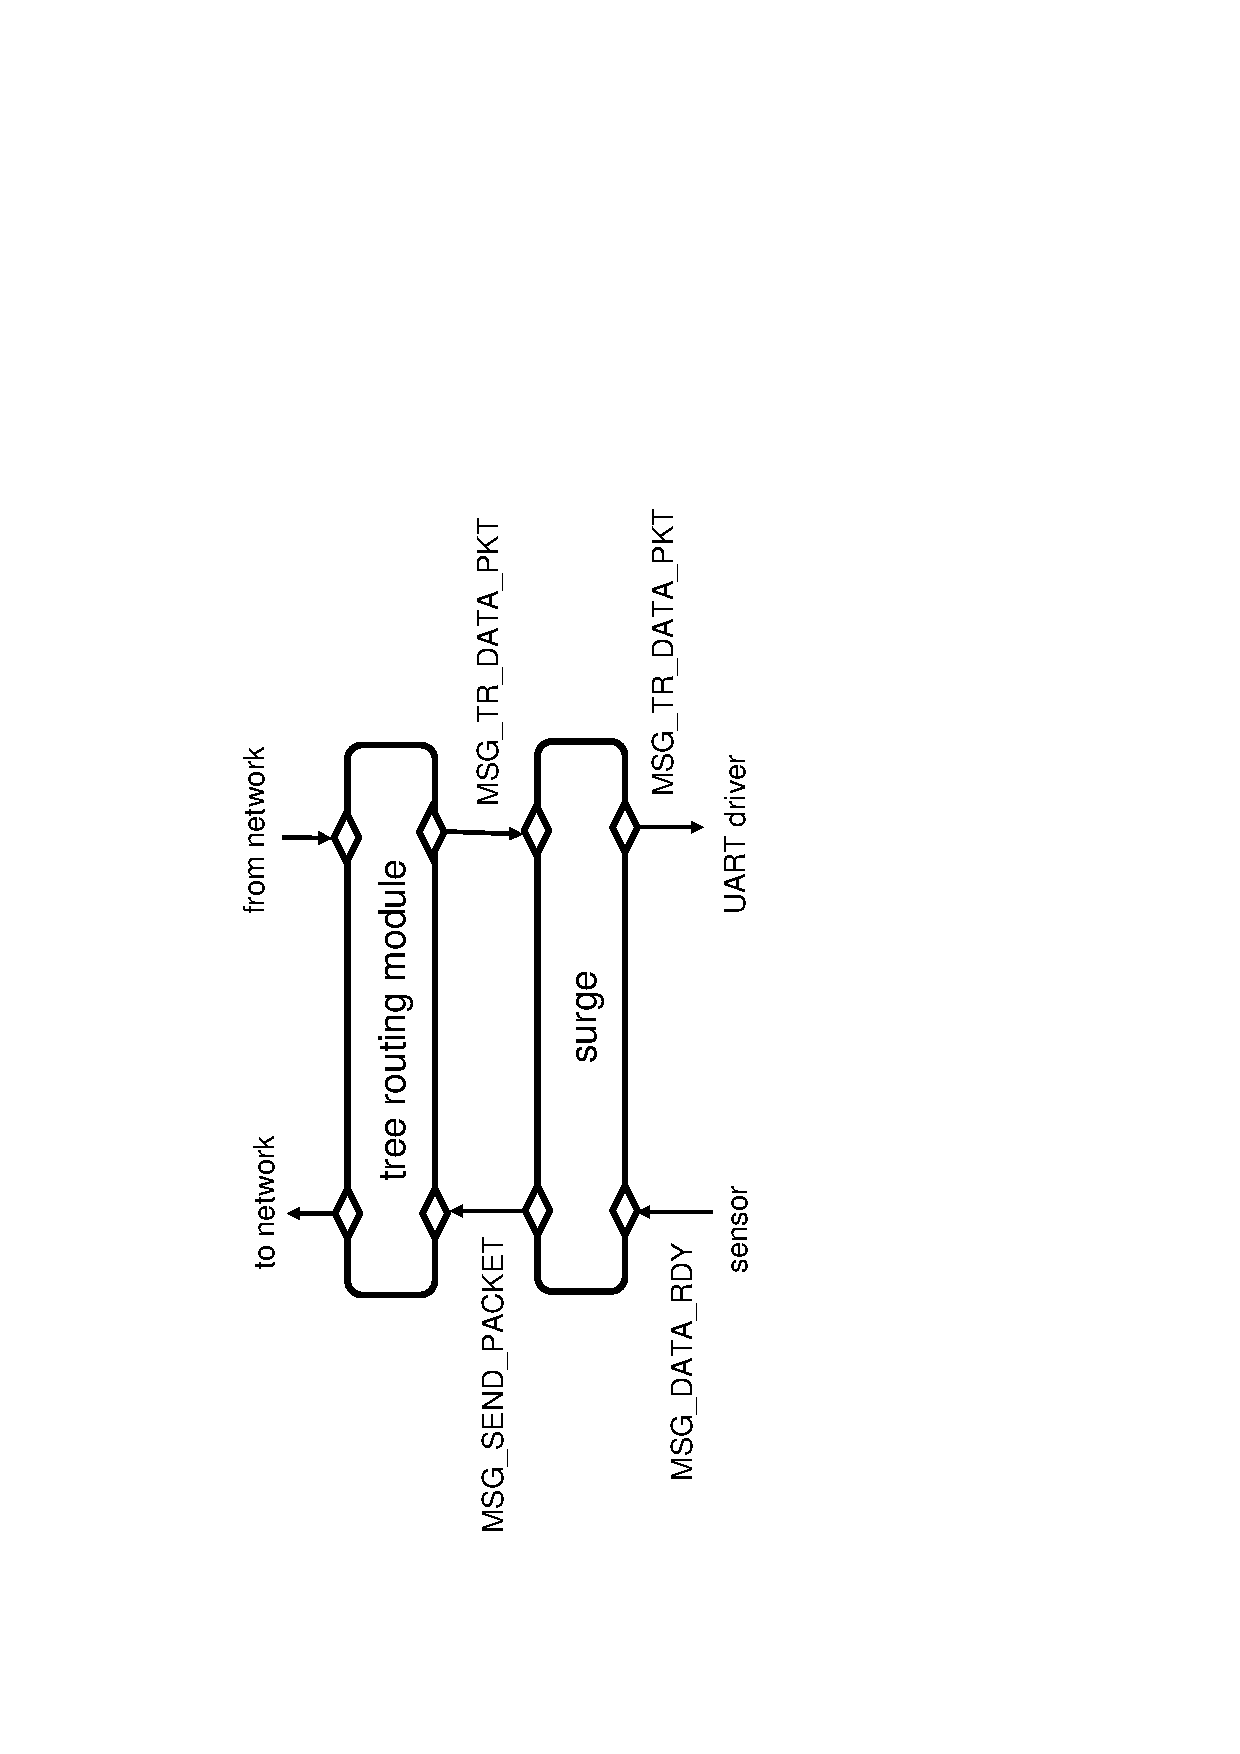
\includegraphics[angle=270,width=4.1in]{surge}
%\caption{{\tt surge} dataflow\label{fig:surge-dataflow}}
%\end{figure}


\subsection{Resource useage in {\tt surge}}

\begin{figure}[t]
\input{surge.c}
\caption{SOS implementation of {\tt surge}\label{fig:surge}}
\end{figure}

Figure~\ref{fig:surge} shows a portion of the SOS module that
implements {\tt surge}, a simple sensor network application that takes
sensor readings and sends the readings over a multihop network to a
base station~\cite{nesC}.  The function {\tt surge\_module} is the
entry point into {\tt surge} for messages from the kernel and from
other modules.  The function takes two arguments: a pointer to the
module's persistent state, which is saved in the kernel, and a pointer
to the current message.  A {\tt switch} statement is used to direct
each message type to an appropriate handler.  The handlers of interest
in this example are for the messages types {\tt MSG\_DATA\_READY} and
{\tt MSG\_TR\_DATA\_PKT}.

A sensor sends the message {\tt MSG\_DATA\_READY} to the surge module
when requested sensor data is ready to be read. The sensor data is
passed as the {\tt data} field of the message, which in general always
contains a message's payload.  Upon receiving this message, the {\tt
surge} message handler allocates a new packet ({\tt ker\_malloc}) to
be sent to the base station and posts a message ({\tt post\_long}) to
the tree-routing module in order to forward the sensor data.  The {\tt
post\_long} call is asynchronous, causing the kernel to package up all
the given arguments into a {\tt Message} structure and to schedule
this message for eventual delivery.

The message {\tt MSG\_TR\_DATA\_PKT} is sent by the tree-routing
module when data is received at the base station node.  Upon receiving
this message, the {\tt surge} message handler confirms that the
current node is the base station.  If so, the message handler forwards
the data to the UART driver via an asynchronous message send ({\tt
post\_net}).

The SOS kernel provides an API for programmers to manage dynamic
memory.  As shown in Figure~\ref{fig:surge}, the {\tt ker\_malloc}
function acts as expected, allocating a new block of memory.  The
kernel also provides a {\tt ker\_free} function for destroying
dynamically allocated memory.  Additionally, ownership of dynamic
memory can be transfered between modules through the messaging
interface provided in SOS.

%
% NOTE (ROY): This is not adding much to the discussion.  10-18-06
%
%In order to provide a simple form of automatic garbage collection for
%dynamically allocated memory, the SOS kernel imposes an {\em
%ownership} model on dynamic memory~\cite{sos}.  Each block of memory
%has a unique owner at any point in time, and the kernel maintains a
%mapping from each block of memory to its owner.  A block's initial
%owner is the module that allocates that block.  For example, the call
%to {\tt ker\_malloc} sets the {\tt surge} module as the initial owner
%of the newly allocated block.  When a module is removed from the
%system at run time, the kernel automatically frees all memory owned by
%that module.

Transfer of dynamic memory ownership occures at the end points of a
message.  First, the owner of a block of dynamically allocated memory
can explicitly {\em release} ownership of that block when it is passed
as the payload in a message.  This is accomplished by setting the
\texttt{SOS\_MSG\_RELEASE} flag in the corresponding {\tt post\_*}
call.  For example, the {\tt surge} module releases ownership of the
newly allocated {\tt pkt} upon sending it to the tree-routing module.
Second, a module can acquire ownership of a message's payload, which
is stored in the {\tt data} field, by calling
\texttt{ker\_msg\_take\_data} on an incoming message.  The function
returns a pointer to the message's payload.  For example, if the
current node is the base station, the {\tt surge} module explicitly
takes ownership of the given message's data under the name {\tt
payload}.

There are four release/take scenarios to consider.  If data is both
released by its sender and taken by its receiver, then ownership of
the data is transferred from the sender to the receiver.  If data is
released by its sender but not taken by its receiver, then the kernel
automatically frees the memory after the receiver's message handler
completes.  If data is not released by its sender but is taken by its
receiver, then the sender keeps ownership of the original message and
the receiver gains ownership of a new block of memory containing a
copy of that data.  Finally, if the data is not released by the sender
and not claimed by the receiver, then the sender keeps ownership of
the original message and the receiver has direct access to
``borrowed'' data for a limited period of time.  This last case is not
generally used in SOS due to the synchronization complications that
can result.


\subsection{Resource useage in {\tt GenericBaseM}}

\begin{figure}[t]
\input{surge.c}
\caption{TinyOS implementation of {\tt GenericBaseM recieve
interface}\label{fig:genericbase}}
\end{figure}


Figure~\ref{fig:genericbase} shows a portion of the TinyOS component that
implements the {\tt receive} event handler for {\tt GenericBase}, an
application that uses a sensor node as a bridge between a base station
and the rest of a sensor network.  The {\tt receive} event handler is
passed in a {\tt TOS\_MsgPtr} pointing to the incoming message and a
flag describing where the message source.

% TODO: Start editing here!!!

% base station~\cite{nesC}.  The function {\tt surge\_module} is the
% entry point into {\tt surge} for messages from the kernel and from
% other modules.  The function takes two arguments: a pointer to the
% module's persistent state, which is saved in the kernel, and a pointer
% to the current message.  A {\tt switch} statement is used to direct
% each message type to an appropriate handler.  The handlers of interest
% in this example are for the messages types {\tt MSG\_DATA\_READY} and
% {\tt MSG\_TR\_DATA\_PKT}.
% 
% A sensor sends the message {\tt MSG\_DATA\_READY} to the surge module
% when requested sensor data is ready to be read. The sensor data is
% passed as the {\tt data} field of the message, which in general always
% contains a message's payload.  Upon receiving this message, the {\tt
% surge} message handler allocates a new packet ({\tt ker\_malloc}) to
% be sent to the base station and posts a message ({\tt post\_long}) to
% the tree-routing module in order to forward the sensor data.  The {\tt
% post\_long} call is asynchronous, causing the kernel to package up all
% the given arguments into a {\tt Message} structure and to schedule
% this message for eventual delivery.
% 
% The message {\tt MSG\_TR\_DATA\_PKT} is sent by the tree-routing
% module when data is received at the base station node.  Upon receiving
% this message, the {\tt surge} message handler confirms that the
% current node is the base station.  If so, the message handler forwards
% the data to the UART driver via an asynchronous message send ({\tt
% post\_net}).
% 
% The SOS kernel provides an API for programmers to manage dynamic
% memory.  As shown in Figure~\ref{fig:surge}, the {\tt ker\_malloc}
% function acts as expected, allocating a new block of memory.  The
% kernel also provides a {\tt ker\_free} function for destroying
% dynamically allocated memory.  Additionally, ownership of dynamic
% memory can be transfered between modules through the messaging
% interface provided in SOS.
% 
% Transfer of dynamic memory ownership occures at the end points of a
% message.  First, the owner of a block of dynamically allocated memory
% can explicitly {\em release} ownership of that block when it is passed
% as the payload in a message.  This is accomplished by setting the
% \texttt{SOS\_MSG\_RELEASE} flag in the corresponding {\tt post\_*}
% call.  For example, the {\tt surge} module releases ownership of the
% newly allocated {\tt pkt} upon sending it to the tree-routing module.
% Second, a module can acquire ownership of a message's payload, which
% is stored in the {\tt data} field, by calling
% \texttt{ker\_msg\_take\_data} on an incoming message.  The function
% returns a pointer to the message's payload.  For example, if the
% current node is the base station, the {\tt surge} module explicitly
% takes ownership of the given message's data under the name {\tt
% payload}.
% 
% There are four release/take scenarios to consider.  If data is both
% released by its sender and taken by its receiver, then ownership of
% the data is transferred from the sender to the receiver.  If data is
% released by its sender but not taken by its receiver, then the kernel
% automatically frees the memory after the receiver's message handler
% completes.  If data is not released by its sender but is taken by its
% receiver, then the sender keeps ownership of the original message and
% the receiver gains ownership of a new block of memory containing a
% copy of that data.  Finally, if the data is not released by the sender
% and not claimed by the receiver, then the sender keeps ownership of
% the original message and the receiver has direct access to
% ``borrowed'' data for a limited period of time.  This last case is not
% generally used in SOS due to the synchronization complications that
% can result.
% 



%%%%%%%%%%%%%%%%%%%%%%%%%%%%%%%%%%%%%%%%%%%%%%%%%%%%%%%%%%%%

\subsection{Static Ownership Checking}

SOS's original concept of ownership as described above
provides a simple form of
garbage collection at run time.
While this can help
reduce the complexity of managing
dynamic memory, it is not sufficient to
prevent memory errors such as dangling pointers and memory leaks.
For example, nothing prevents a module from freeing some memory while
another module (or even the same module) still has a pointer to that
memory.  If that pointer is ever accessed later, an invalid dereference
will result.  Further, garbage collection introduces the potential for
more dangling pointer errors, since the removal of a module implicitly
frees the memory it owns, even if other modules have pointers to that
memory.

%% The basic problem is that SOS's intuitive concept of ownership is
%% not enforced.  There is no guarantee that
%% a program's ownership directives and
%% annotations are consistent with the rest of the program.  Further,
%% there is no explicit notion of what it means to be consistent, namely the
%% rights and responsibilities of owners and non-owners with respect to
%% dynamic memory.  Instead, the burden is on the programmer to ensure
%% that the implicit ownership protocol is properly respected.

In this work, we augment SOS's ownership directives to
provide a protocol governing
memory management that is sufficient to ensure the absence of
memory errors.
Our protocol makes explicit a common programming idiom in
sensor-network systems, whereby data is rarely shared but instead
follows a producer/consumer model.
We have built a tool that checks for violations of this protocol on
each SOS module at compile time.

Informally, the rules of the protocol can be stated as
follows:
\begin{itemize}

\item A module may only manipulate the memory that it owns.

\item A module that takes ownership of a block of memory (either
  through {\tt ker\_malloc} or {\tt ker\_msg\_take\_data}) must either
  free that memory, release it, or store it in the module's
  persistent state.

\item A module may only free or release memory that it owns.  After a module
  frees or releases memory, it may not access or update that memory.
\end{itemize}
Because only the owner can manipulate or free its
memory, dangling pointers are avoided.  Because all memory must be
either freed, released or persistently stored by its owner,
memory leaks are avoided.


\subsection{{\tt surge} Revisited}

Our tool is able to validate at compile time that the
{\tt surge} module properly obeys the ownership protocol.
The {\tt MSG\_DATA\_RDY} message handler
allocates {\tt pkt} and takes
ownership. This pointer is then dereferenced in order to provide the
sensor data
to be sent up the routing tree.
This pointer manipulation is safe since the module has ownership.
The module then
releases ownership by posting {\tt pkt} to the tree routing module
using the {\tt SOS\_MSG\_RELEASE} tag.  After this release, the
module does not access
{\tt pkt} again and does not store it, ensuring that access to the
pointer is indeed released. 

The handler for {\tt MSG\_TR\_DATA\_PKT} also conforms to the
protocol.   When the current
node is the base station, the handler explicitly acquires ownership of
the message's data
using {\tt ker\_msg\_take\_data}.  This allows the module to
manipulate the data and to pass it to
the UART.  The {\tt post\_net} call
explicitly releases the data, fulfilling the module's obligation to
that data.   After the release, the data
is no longer accessed or stored.

While the {\tt surge} code is correct, small changes to the code can
easily cause problems to occur at run time, and our static checker
catches these potential errors.  For example, suppose the handler for
{\tt MSG\_DATA\_READY} did not release ownership of {\tt pkt} by setting the 
{\tt SOS\_MSG\_RELEASE} flag in the call to {\tt post\_long}.
In that case, the module would leak the memory allocated for {\tt pkt}.
Indeed, our checker flags this
modified version of the code as erroneous, since {\tt surge} would not be
freeing, releasing, or storing the data for which it has taken ownership.

\subsection{Function Attributes}

%% The next section details the way in which our tool conservatively
%% ensures at compile time that SOS modules obey this protocol.  The
%% heart of the checker is a suite of dataflow analyses that statically
%% approximate the dynamic ownership relationships.  
%% So far, we have described the analysis for the {\em intra-procedural case},
%% i.e., when there are no function calls.
Our analysis is {\em modular}:  
each function in a module is analyzed in isolation.  To make checking
of a function body precise in the presence of calls to other
functions, we employ
{\em ownership attributes} for function headers that capture the memory-related
behavior of a called function.
We add two attributes to the SOS API: {\tt sos\_claim} and {\tt sos\_release}.
A formal parameter or return value
that has the {\tt sos\_claim} attribute indicates that the
caller must take ownership of the associated memory after a call.
This annotation, for example, would be used to annotate a function that
wraps a call to {\tt ker\_malloc}, allowing that function's callers to
be properly checked without access to the function's implementation.
Similarly, an {\tt sos\_release} attribute on a formal parameter
%
indicates that ownership of the parameter is transferred from the caller of the
function to the callee.
%indicates that the parameter's contents are either released or freed
%(directly or indirectly) by the function.
%
If a parameter does not have an ownership attribute, memory ownership
is unchanged.
%% Our tool makes use of ownership attributes to precisely check callers
%% of a function.  
Our tool ensures that these attributes are employed wherever 
necessary, when checking the implementation of each function. 
%
%% Attributes do not need to reside in the code.  An annotation configuration
%% file can be used by the checker to insert attributes during analyses.  The
%% annotations in this configuration look like:
%% %
%% \begin{footnotesize}
%% \begin{verbatim}
%% add annotations "ker_malloc" [Some "sos_claim"; None; None];
%% \end{verbatim}
%% \end{footnotesize}
%% %
%% specifying that the {\tt sos\_claim} attribute should be added to the 
%% data returned by {\tt ker\_malloc} and that the two formal parameters need
%% no additional ownership attributes.  Our tool assumes that functions not described in
%% the annotation configuration need no other attributes added to them.  
In practice, we have found that a small set of annotations
is sufficient for precise analysis.
%% to obviate the need for explicit attributes annotations in user code.

\subsection{Generality}

Memory errors in SOS were the original motivation for our work.
Further, the existing ownership directives for dynamic
memory in SOS facilitated the creation of our tool.  However, we stress that
the underlying protocol that we enforce
is completely independent of both SOS and of
memory in particular.  For example, it would be straightforward to
apply our tool to track resources other than memory in SOS, and
we could similarly port our tool to enforce an ownership protocol on
nesC's static buffers rather than
SOS's dynamic memory.


\section{The Lighthouse Tool}
\label{sec:alg}



We have instantiated our approach to static checking of dynamic resource
management in Lighthouse, a tool for ensuring proper ownership of dynamic
memory in SOS programs.
%
The tool employs a suite of dataflow analyses to enforce the three rules
described in Section~\ref{subsec:owner} on each function.
%
This section overviews the usage and implementation of Lighthouse.



\subsection{Ownership Annotations}


Lighthouse depends on programmer-specified {\em ownership annotations} to
specify when ownership of a block of memory should transfer from one
component to another.
%
These annotations provide a ``spec'' for each function, indicating its
preconditions and postconditions with respect to memory ownership.  
%
This spec then enables precise modular checking of functions.  
%
Each function body is checked to ensure the postconditions on exit, under
the assumption that the preconditions hold on entry.  
%
The function is also checked to obey the three rules constituting the
ownership discipline, defined earlier.  
%
Each caller is separately checked to ensure the callee's preconditions
before the call, and it may assume the callee's postconditions after the
call.



Two ownership annotations are used to describe changes of memory ownership
resulting from function calls: {\tt lh\_claim} and {\tt lh\_release}.
%
The {\tt lh\_claim} annotation states that the caller of the function will
take ownership of the memory pointed to by the annotated formal parameter or
annotated return value, and therefore that the function body must release
it.
%
For example, the SOS kernel's \code{ker\_malloc} function has the {\tt
lh\_claim} annotation on its return value, to indicate that it returns
dynamically allocated memory that the caller will own.
%
Conversely, the {\tt lh\_release} annotation states that the caller of the
function will release ownership of the memory pointed to by the annotated
formal parameter, and therefore that the function body must take ownership
of this memory.
%
For example, the formal parameter of the SOS kernel's \code{ker\_free}
function has the {\tt lh\_release} annotation.



Our ownership discipline defined earlier relies on the notion of a {\em
persistent store}:  each component is assumed to own the data in its
persistent store and can properly ``release'' owned data into this store.
%
All global and static variables declared with a component are assumed by the
analysis to be part of the component's persistent store.
%
A third and final annotation, {\tt lh\_store}, is used to denote formal
parameters of functions that can also be considered part of the persistent
store.
%
An example usage of {\tt lh\_store} is to annotate the \code{state}
parameter of a module's message handler in SOS.
%
As described earlier, this parameter points to the persistent store
allocated and maintained by the SOS kernel for a module.



Annotations typically reside in an external configuration file listing a
function name and the corresponding annotations for the return value and
formal parameters.
%
Only functions that require annotations need to be included within this
configuration file.
%
Annotations can also be included directly in the source code as GCC
attributes decorating the prototype of a function.
%
In practice we have found that a small set of annotations, \numannote for
the complete evaluation of SOS, is sufficient for precise analysis. 



The ability to perform checking modularly allows application writers to
obtain early feedback about the correctness of their resource management,
without requiring access to the rest of the system.  
%
This is particularly important in a system like SOS, in which modules can be
linked and unlinked dynamically.  
%
In such a setting, the ``rest'' of the system is a moving target, so it is
not really possible to consider an approach based on whole-program analysis.



\subsection{Implementation Overview}



Lighthouse is implemented in the CIL front end for C~\cite{CIL}, which
parses C code into a simple intermediate format and provides a framework for
performing analyses on the intermediate code. 
%
Lighthouse takes as input a preprocessed C file and prints out warning
messages similar to those produced by a C compiler when suspect code is
identified.
%
The analysis does not modify the preprocessed code, so it can be trivially
called from a makefile between the preprocessing and code generation stages
of compilation.



The Lighthouse analysis traverses each function's control-flow graph (CFG)
in isolation, which conservatively represents all possible execution paths
through the function.  
%
During this traversal, Lighthouse triggers two major dataflow analyses to
detect potential errors:



\begin{itemize}



\item Whenever a node in the graph is encountered that allocates or takes
ownership of a block of memory, Lighthouse invokes a dataflow analysis to
ensure that every path from this node to the function exit frees, stores, or
releases ownership of the memory exactly once.  
%
If this property is not satisfied, Lighthouse reports a possible memory
leak.



\item Whenever a node in the graph is encountered that frees or releases
ownership of a block of memory, Lighthouse invokes a dataflow analysis to
ensure that no path from this node to the function exit accesses the memory.  
%
If this property is not satisfied, Lighthouse reports a possible dangling
pointer error.



\end{itemize}



These two analyses also serve to check that a function meets its spec.  
%
For the purpose of the Lighthouse traversal over a function's CFG, the
function's entry node is considered an allocation point for all parameters
with the {\tt lh\_release} annotation, and the function's exit node is
considered a release point for all parameters and return values with the
{\tt lh\_claim} annotation.  



\subsection{Pointer Aliasing}



The analysis described above requires knowledge of the memory pointed to by
a function's pointers.  
%
As usual, this is statically approximated by an {\em alias analysis}, which
determines whether two different pointers store the same memory location at
a given program point.  
%
Two standard approximations to the true dynamic alias information are {\em
must-alias} analysis and {\em may-alias} analysis.  
%
A must-alias analysis underapproximates the dynamic alias relations:  if a
must-alias analysis determines that $x$ and $y$ alias at a particular
program point, then they definitely alias at that point in any program
execution.  
%
A may-alias analysis overapproximates the dynamic alias relations:  if a
may-alias analysis determines that $x$ and $y$ {\em cannot} alias at a
particular program point, then they definitely do not alias at that point in
any program execution.



Lighthouse requires both kinds of static alias approximations.  
%
In the first dataflow analysis described above, alias information is used to
ensure that something definitely happens, namely that an allocated resource
is eventually released.  
%
Therefore, in this case we approximate the true alias information with
must-alias information.  
%
In the second dataflow analysis described above, alias information is used
to ensure that something definitely does not happen, namely an access to a
released resource.  
%
Therefore, in this case we approximate the true alias information with
may-alias information.



We have built a simple flow-sensitive must-alias analysis for use by
Lighthouse.  
%
For the may-alias analysis, we use a fast flow-insensitive analysis provided
by the CIL framework.  
%
Obtaining precise alias information at compile time is notoriously
difficult, and this limitation is the principal cause of false positives for
our analysis.
%
For example, CIL's may-alias analysis does not distinguish among the fields
of a structure, instead considering them to always potentially alias one
another.  
%
Both alias analyses can be imprecise in the presence of linked data
structures.



\subsection{Limitations}



As we demonstrate in the next section, our checker is useful for detecting
violations of the ownership protocol on real sensor network code.  
%
However, the checker is not guaranteed to find all such violations.  
%
In other words, the checker can be used for finding memory errors but not
for guaranteeing the absence of all memory errors.  
%
The checker's false negatives come from three sources.



First, the checker does not precisely handle all of the unsafe features of
the C programming language.  
%
For example, pointer arithmetic is not statically analyzed.  
%
Instead, an expression of the form $p+i$, where $p$ is a pointer and $i$ is
an integer, is simply treated as if it refers to the same block of memory as
$p$.  
%
If $p+i$ in fact overflows to another block of memory at run time, the
checker's assumption can cause it to miss errors.  
%
These kinds of {\em memory safety} assumptions are standard for C-based
program analyses.



Second, there is a design choice about how to treat resource parameters that
are not annotated with {\tt lh\_release}.  Technically the ownership
protocol disallows these resources from being accessed at all, since the
receiving component is not the owner.  
%
Lighthouse does not currently enforce the requirement that a component only
access a resource that it owns.
% 
This design decision provides a seamless adoption path for Lighthouse on
existing systems.  
%
Programmers can incrementally add annotations to refine the quality of the
analysis without suffering from excessive numbers of false positives.
%
This decision also provides a mechanism for allowing patterns of resource
sharing that are in fact safe but not supported by the ownership discipline,
for example when a component temporarily ``borrows'' data from another
component within a bounded scope.
%
The cost of this flexibility is the potential to miss real resource
management errors.
%
However, the checker still ensures that a function does not access a
resource that has earlier been released by the function, thereby detecting
memory leaks.



Third, our modular checker does not consider the overall order in which
messages will be received by a component.  
%
However, event orderings can affect the correctness of ownership tracking
when a resource is accessed via the persistent store.
%
For example, consider a component that responds to three events: $\create$
causes the component to allocate a block $b$ and store it into the
component's persistent store, $\access$ causes the component to access block
$b$ via the store, and $\delete$ causes the component to deallocate block
$b$ from the store.  
%
The component avoids dangling accesses to $b$ and leaks of $b$ as long as
the temporal sequence of events follows the regular expression $($ $\alloc$
$\access^*$ $\delete$ $)^*$.  



Lighthouse currently only tracks data locally within each event handler.  
%
When performing this tracking, the tool assumes on entry that all data in
the persistent store is owned by the component.
%
The tool similarly considers a resource to be properly released when it is
placed in the persistent store.  
%
These assumptions allow each of the three event handlers in our example to
pass all checks.  
%
Nonetheless, dynamic memory errors can still happen, for example if an
$\access$ event ever occurs before the $\alloc$ event.  
%
Our assumptions provide a practical point in the design space that allows
each event handler to be usefully checked for local violations of the
ownership protocol.  
%
Handling inter-component relationships and application-level protocols is
something we plan to pursue in the future, leveraging recent work on {\em
interface synthesis} for software components~\cite{AlurPOPL05,HJM05}.


\section{Evaluation}
\label{sec:eval}

This evaluation examines to what extent this type of tool is needed
within the sensor network community and how effetive it is at
isolating problems within sensor network systems.  Our evaluation
focused on the SOS operating system, using the public CVS archives to
supply programs for analysis.  SOS applications are made up of small
user modules that can be combined into larger programs.  These modules
run ontop of a well defined kernel and are developed using an API
supplied by this kernel.


\subsection{Quantifying Dynamic Memory Usage in SOS}

Of interest is the prevalence of dynamic resource management within
sensor network systems.  TinyOS displays this through buffer swapping
within messaging stacks and more general message queues.  Within SOS
this is seen through memory buffer management.  

Focusing on SOS, we quantify the usage of operations that manipulate
memory ownership within the SOS operating system.  The SOS API
includes a number of functions that manipulate memory.  These
functions are used to allocate, free, and transfer ownership of blocks
of memory.  

The CVS head from October 2006 reveals 36 modules totaling 5824 lines
of source code.  Within this sample there are 178 lines of code
calling a function that manipulates memory, or one such function call
for every 32 lines of code.  Looking at all historic version of all
SOS modules reveals that this frequency has not changed signifacntly
over time.  These findings indicate that memory management has been
and continues to be an important part of resource management in SOS.


\subsection{Validating SOS End-User Modules}

Two additional questions arise as a result of the observation that
memory is frequentnly manipulated as a resource in SOS.  These
questions are:
%
\begin{itemize}
%
\item Do programers have problems properly using the resource
managment?
%
\item Would the analysis described in this paper help with
those problems?
%
\end{itemize}

To address these questions we ran our tool on all versions of all SOS
end-user modules contained within the CVS repository to demonstrate
how it would fit into an everyday development cycle.  For this
analysis, we only consider the first occurrence of a particular bug
withing a program, even if the bug lasts through multiple consecutive
versions of a particular module.  We applied the checker to every
historic version of each user module included in the SOS CVS
repository that would compile for the \code{mica2} target.  The 48
available modules resulted in a total of 213 unique versions.
%
An external configuration of 24 function annotations was used for this
analysis.  
%
Additionally, local store annotations were added to 9 module versions
and a change to the core SOS API from the summer of 2006 required
changing the value of a constant in 6 module versions.


\begin{table}
\caption{Warnings in SOS user modules}
%
\label{tab:module}
\centering 
\begin{tabular}{| l | r |}
    \hline 
    Verified memory leaks identified by analysis & 8 \\
    \hline
    False memory leaks identified by analysis & 8 \\
    \hline 
    Verified dangling pointers identified by analysis & 0 \\
    \hline 
    False dangling pointers identified by analysis & 9 \\
    \hline 
\end{tabular} 
%
\end{table}

Of the 213 modules analyzed, 13 of the modules generaed warnings for a
total of 25 warnings.
%
Each warning was examined by hand and classified as an actual error or
a false positive; the results are presented in Table~\ref{tab:module}.  
%
Eight of the warnings turned out to be real memory leaks in the code.
%
The 17 remaining warnings were further classified to better understand
the sources of imprecision in the current implementation of the
checker.  

\smallskip\noindent{\bf Memory leak false positives.}

False positives from memory leaks came from two different sources.
Five of the false positives resulted from a conservative assumption
made by the must alias analysis used within the checker.  The analysis
assumes that functions can change what data is referenced by a formal
parameter.  This results in required must alias information being lost
in these cases.  The analysis can easily rank these as probable false
positives if the end user wishes to see more likely errors first.  The
other three memory leaks are the result of linked list data structures
that the must alias analysis is unable to properly reason about.  

\smallskip\noindent{\bf Dangling pointer false positives.}

The nine dangling pointer false positives result from limitations of
the flow-insensitive and field-insensitive may analysis.  Elimination
of these false positives would require a more accurate may analysis.
Modern sensor network applications are made of small components that
effecivly limit the scope of variables.  This opens the door to using
context sensitive analysis that suffer from scaling limitations in
more general domains.


\subsection{Validating the SOS Kernel}

\begin{table}
\caption{Warnings in the SOS kernel}
%
\label{tab:kernel}
\centering 
\begin{tabular}{| l | r |}
    \hline 
    Verified memory leaks identified by analysis & 2 \\
    \hline
    False memory leaks identified by analysis & 22 \\
    \hline 
    Verified dangling pointers identified by analysis & 0 \\
    \hline 
    False dangling pointers identified by analysis & 11 \\
    \hline 
\end{tabular} 
%
\end{table}


We ran a similar experiment on all code required to build the core the
SOS kernel for the \code{mica2} target.  This configuration consists
of approximately 9000 lines of source code and required analyzing 40
source files, of which 35 generated warnings.  A detailed breakdown of
these warnings is provided in table~\ref{tab:kernel}.

\mynote{ROY: This paragraph is very awkward.  It needs to be
rephrased.} 
%
The two actual memory leaks represent an interesting type of error.
These leaks resulted from functions that released a formal parameter,
except in exceptional cases where an error code is returned to the
user.  It is more accurate to say that these functions do not leak
memory, but rather conditionally release memory.  However user code
treats these functions as unconditional releases, not bothering to
check the return vaules.  Since changing these two functions would
result in a number of errors in user code, we assumed that the two
kernel functions are incorrect.

A second point of interest is the different rates of false positives
reported for user modules and for the kernel.  User modules resulted
in approximately one false positive for every 1650 lines of source
code.  The kernel saw a much higher frequency at approximately one 
false positive for every 270 lines of source code.  

A large contributor to this increased rate of false positives within
the kernel are the bottom layer functions implementing management of
memory in SOS.  These functions manipulate memory in a manner that
does not conform to the model assumed for the analysis.  For example,
the function \code{ker\_msg\_take\_data} is annotated to denote that
it returns dynamically allocated memory, but the analysis warns that
no such memory is returned.  This is because the function directly
accesses the internal data structures of the SOS memory manager to
return a pointer to dynamically allocated data, rather than using an
annotated interface such as \code{ker\_malloc}.
%
\mynote{ROY: What is the point of this paragraph?}


% ROY (11/04/06):
% This does not seem to stand on its own.  For now I will simply leave
% the allision to this challenge as a point for the conclusion.
%
% \subsection{Comments}
% 
% A third source of false positives arises from application-level
% protocols that ensure memory is used correctly across multiple
% invocations of the module's message handler, but which cannot be
% validated modularly.

\subsection{A Memory Leak in SOS}
\label{ss:tale}

\begin{figure}[tp]
\begin{footnotesize}
\begin{verbatim}
mod_op = (sos_module_op_t*) ker_msg_take_data(msg);
if(mod_op == NULL) return -ENOMEM;
if(mod_op->op == MODULE_OP_INSMOD) {
    existing_module = ker_get_module(mod_op->mod_id);
    if(existing_module != NULL) {
        uint8_t ver = sos_read_header_byte(
                existing_module->header,
                offsetof(mod_header_t, version));
            if (ver < mod_op->version) {
                ker_unload_module(existing_module->pid, 
                        sos_read_header_byte(
                        existing_module->header,
                        offsetof(mod_header_t, version)));
            } else {
                return SOS_OK;
            }
        }
    ret = fetcher_request(KER_DFT_LOADER_PID,
            mod_op->mod_id,
            mod_op->version,
            entohs(mod_op->size),
            msg->saddr);
    s->pend = mod_op;
    ker_led(LED_RED_TOGGLE);
    return SOS_OK;
}
return SOS_OK;
\end{verbatim}
\end{footnotesize}
\label{fig:leak}
\caption{A memory leak in an SOS module.}
\end{figure}

This section examines the SOS loader, a core part of SOS that allows
users to dynamically add modules to a running system and that is
known to have caused stability problems for developers in the past.
We used the checker to see if such a tool could have eased development
pains.

In mid-October 2005 the block of code shown in Figure~\ref{fig:leak}
was checked into CVS as part of {\tt loader.c} and introduced a memory
leak into the loader.  All paths through this block of code leak the
{\tt mod\_op} pointer, which the module acquires ownership of through
{\tt ker\_msg\_take\_data}.  This code results in the following
warning from the checker:

\begin{footnotesize}
\begin{verbatim}
Error: Expression mod_op is not stored after instruction #line 125
mod_op = (sos_module_op_t *)ker_msg_take_data((unsigned char)18, msg);
\end{verbatim}
\end{footnotesize}

After three additional revisions that do not significantly modify or
fix the memory leak, a fourth revision was made in mid-December 2005.
This revision expands the functionality of {\tt loader.c} and breaks
the code up into smaller functions:

\begin{footnotesize}
\begin{verbatim}
sos_module_op_t *mod_op;
if (msg->saddr == ker_id() || s->pend) {
    return SOS_OK;
}
mod_op = (sos_module_op_t*) ker_msg_take_data(msg);
if(mod_op == NULL) return -ENOMEM;
switch(mod_op->op){
case MODULE_OP_INSMOD:
    return module_op_insmod(s,msg,mod_op);
case MODULE_OP_RMMOD:
    return module_op_rmmod(s,msg,mod_op);
}
return SOS_OK;
\end{verbatim}
\end{footnotesize}

This code again causes our checker to warn about the memory leak:

\begin{footnotesize}
\begin{verbatim}
Error: Expression mod_op is not stored after instruction #line 186
mod_op = (sos_module_op_t *)ker_msg_take_data((unsigned char)18, msg);
\end{verbatim}
\end{footnotesize}

Clearly {\tt mod\_op} is still being leaked if {\tt mod\_op->op} does
not find a matching case in the {\tt switch} statement.  Further,
adding the {\tt sos\_release} attribute to the third formal parameter
of the functions {\tt module\_op\_insmod} and {\tt module\_op\_rmmod}
and rerunning the checker reveals that both of these functions also
leak {\tt mod\_op}!

A day later, eight weeks after the memory leaks were first introduced,
these memory leaks were found and fixed:

\begin{footnotesize}
\begin{verbatim}
sos_module_op_t *mod_op;
if (msg->saddr == ker_id() || s->pend) {
    return SOS_OK;
}
mod_op = (sos_module_op_t*) ker_msg_take_data(msg);
if(mod_op == NULL) return -ENOMEM;
switch(mod_op->op){
case MODULE_OP_INSMOD:
    return module_op_insmod(s,msg,mod_op);
case MODULE_OP_RMMOD:
    return module_op_rmmod(s,msg,mod_op);
}
ker_free(mod_op);
return SOS_OK;
\end{verbatim}
\end{footnotesize}

As shown above, a call to {\tt ker\_free} has been added before the
final {\tt return}, in order to properly dispose of {\tt mod\_op}.
The functions {\tt module\_op\_insmod} and {\tt module\_op\_rmmod}
similarly free their third argument.  The CVS log message simply reads
``fixed another memory leak.''






\section{Related Work}
\label{sec:related}

\subsection{Sensor Network Analysis Research}

The memory manager in the SOS operating
system~\cite{sos} performs basic memory ownership tracking to clean
the system after module removal.
%
However, the burden remains on the end user to prevent memory leaks in
active modules and to not dereference invalid pointers.
%
Our work grew out of a desire to prevent these kinds of errors from
occurring in SOS applications.



Dynamic checking of sensor network systems has become a popular technique to
improve system reliability and find system errors.
%
Recent work on Safe TinyOS, UTOS~\cite{regehr06memory} and software fault
isolation for embedded processors~\cite{kumar07system} uses static analysis
to insert run-time checks ensuring memory protection for sensor-network
systems.
%
Interface contract monitoring~\cite{archer07interface} interposes a thin
layer between interface clients and implementers, and has proved effective
in finding bugs in TinyOS programs.
%
These approaches provide valuable feedback to developers when an executing
system misbehaves.
%
In contrast to these works, the static analysis in Lighthouse focuses on
alerting developers to problems at compile time.



Sensor network platforms include support for static checking targeting
other classes of errors.  
%
The nesC~\cite{nesC} language used in TinyOS employs a whole-program
analysis to statically detect race conditions and
galsC~\cite{TinyGALS,galsC} employs an analysis to ensure the type safety of
connections between components.  



A complementary approach to improving the reliability of sensor network
software is through new language abstractions.  
%
Researchers have explored language support for component-based
programming~\cite{TinyOS,nesC,galsC}, region
abstractions~\cite{conf/mobisys/WhitehouseSCB04,conf/nsdi/WelshM04},
component composition~\cite{conf/sensys/GreensteinKE04}, and programming in
the aggregate~\cite{1052213,conf/dcoss/GummadiGG05}.
%
New language constructs enable easier expression of certain programming
idioms, often making programs more amenable to static checking.  
%
Our tool currently analyzes ordinary C programs, since that is the language
that SOS employs, but it would be interesting to explore ways to leverage
specialized language constructs to improve the tool's effectiveness.



\subsection{Traditional Systems Analysis Research}



Static analysis has long been used to find bugs in traditional systems.
%
Dedicated languages, such as Metal~\cite{engler00checking}, are used to
compose custom compiler extensions to verify properties at compile time.
%
Such properties can even be inferred from the code
itself~\cite{kremenek06from}.
%
Clouseau~\cite{heine03practical} uses a whole program constraint analysis to
ensure that dynamically allocated memory is freed exactly once in C and C++
programs.
%
Our work contrasts with these approaches by focusing on creating an
understandable programming discipline.
%
This is accomplished using explicit lightweight specifications that increase
developer visibility into the analysis and obviate the need for
interprocedural analysis.
%
Other technical differences exist between the systems.
%
While our general ownership discipline could be described using the Metal
language, Lighthouse provides a stronger analysis by explicitly considering
aliasing, a challenge not handled within Metal.
%
Unlike Clouseau, our work detects dangling pointers in addition to memory
leaks.




Recent work in the programming languages community explores the concept of
ownership types~\cite{ownership,ownership2,BoyapatiEtAl02,aliasjava} for
object-oriented languages. 
%
Ownership types designate an owner object for each object, and the static
type system ensures access to an object goes through its owner.
%
Related work on confined types~\cite{confined1,confined2} provides a more
static form of confinement, in which an object is guaranteed not to escape a
particular static scope.



Our work provides a static notion of ownership analogous to that of confined
types:  all accesses to a given resource may only occur within the static
scope of its owning module.  
%
On a technical level, however, the foundation of our work is quite distinct
from that of both ownership types and confined types, as we rely on dataflow
analysis rather than on type systems.  
%
Our use of dataflow analysis is necessary in order to safely accommodate
dynamic transfer of ownership, which the systems described above lack.  
%
Ownership transfer is critical in practice for sensor network applications,
for example it is needed to properly account for split-phase operations.  
%
Although recent work has explored a form of transfer in the context of
ownership type systems~\cite{DBLP:conf/ecoop/BanerjeeN05}, that work
requires programmers to provide detailed assertions about ownership, and
these assertions are proved as part of a more general program specification
and verification framework.



There have been several proposals for a form of {\em unique} or {\em linear}
pointer~\cite{Boyland:2001:ABU,aliasjava,Wad90:linear}, which is guaranteed
to be the only reference to its referent.  
%
These systems sometimes include a form of transfer of uniqueness from one
pointer to another.
%
For example, a {\tt unique} pointer in AliasJava~\cite{aliasjava} can be
transferred as long as a dataflow analysis shows that the original pointer
is no longer accessed after the transfer.  
%
Our tool does not enforce a uniqueness requirement.
%
Instead, a resource may have any number of aliases from within its owning
component, which is less restrictive and sometimes necessary in practice.
%
At the same time, transfer is still safely allowed, as long as none of these
aliases are accessed after the transfer.



A language extension to C\# called Sing\# provides a {\em channel} construct
for message-based communication, and the Singularity operating system uses
Sing\# channels for communication among
processes~\cite{fahndrich06language}.  
%
Sing\# employs a type system for channels based on the Vault
language~\cite{Vault,adoption-focus}, which provides a sophisticated form of
linear types, to enforce ownership invariants on data buffers passed among
processes.  
%
This includes the use of programmer-defined channel {\em contracts} to
specify and check ownership transfer.
%
Lighthouse enforces a similar ownership discipline on dynamic memory in SOS,
but at a very different point in the design space.  
%
Rather than devising a new language and type system, our approach works
seamlessly with standard languages and tool chains for sensor-network
programming in a lightweight manner.  
%
Of course, a language solution like Sing\# has the potential to be more
expressive and to provide stronger guarantees, by enforcing a stylized
programming model.



\section{Conclusion}
\label{sec:conc}

Systems programming APIs for networked embedded systems applications
are getting more expressive as the applications become more
sophisticated.  This necessitates a programming environment that
supports program development by providing automated compile-time
checkers for proper API usage.  Support for such validation is
particularly important in the sensor network domain.  First,
sensor network software is intended to run under resource constraints
and unpredictable environments, making them more prone to error.
Second, the cost of fixing a bug in the field is
high.  Third, networked embedded systems come with somewhat limited
debugging support, making it extremely difficult to reason about the
cause for a failure in the field.

This paper is our first step toward providing static analysis tools
that capture common programming idioms in networked embedded systems.
We have focused on dynamic resource management initially, since our
experience with SOS suggests that improper memory management is a
common source of hard-to-debug problems.  We have demonstrated how our
approach can effectively find memory errors even in code written by
systems experts.  Lighthouse is publicly available for those wishing to
experiment with the system.

In the future, we would like to augment the techniques in this paper
with support for reasoning about application-level protocols
\cite{AlurPOPL05,HJM05} as well as concurrency issues.  Ultimately,
our goal is to provide a systems programming environment where many
common classes of bugs are automatically detected at compile time.  We
believe such early feedback will help increase the productivity of
sensor network programmers and the reliability of their software.




{\small 
\bibliographystyle{plain}
\bibliography{sw,sos,references}

}

\end{document}


